\graphicspath{{../img/intro/}}

\chapter{Introduction}
The rapid proliferation of data across various domains and artificial intelligence applications has led to an explosion of high-dimensional datasets. As these collections grow, encompassing millions or even billions of data points, the challenge becomes how to efficiently process, analyze, and retrieve relevant information. Many data-driven applications, from machine learning models to recommendation systems, rely on effective interaction with these datasets to extract insights and knowledge on demand, with vector search being a core operation.

While traditional vector search approaches such as tree-based and hash-based methods attempt to execute this task efficiently, they often fail to deliver satisfactory performance at scale. Over the last decade, graph-based methods have emerged as a leading solution for efficient vector search, offering high recall and impressive query efficiency. However, existing graph-based structures still face significant challenges when it comes to scaling efficiently to massive collections.

This thesis addresses these challenges by proposing novel methods that advance the state of the art in high-dimensional similarity search. We introduce ELPIS, a new approach for in-memory ng-approximate high-dimensional vector search that leverages both tree and graph structures, combining their strengths to overcome mutual limitations and outperform state-of-the-art methods in terms of latency, while offering competitive throughput. Additionally, we propose a new taxonomy that categorizes state-of-the-art graph-based approaches according to key paradigms, providing insights into the strengths and weaknesses of each. Finally, we present a novel graph-based approach that improves indexing scalability and query performance over existing methods.

In this chapter, we first provide an overview of the similarity search problem and the main data types addressed in this work, followed by a summary of the key contributions of this thesis.
\clearpage 

%\section{Problem Overview}
\section{Overview}
\label{sec:overview}
Vector search is a backbone operation at the core of many essential data analytics tasks. It supports recommendation~\cite{conf/kdd/wang2018,amazon}, 
information retrieval~\cite{conf/williams2014}, clustering~\cite{journal/JMLR/bubeck2009,journal/pattrecog/Warren2005}, 
classification~\cite{classification,pros},
and anomaly detection~\cite{discord,norma,series2graph,landmines,nba,landmines,DBLP:journals/datamine/LinardiZPK20,DBLP:journals/pvldb/BoniolPPF21,DBLP:journals/pvldb/PaparrizosKBTPF22,DBLP:journals/pvldb/PaparrizosBPTEF22} across various scientific and business domains, including bioinformatics~\cite{biof1,biof2}, 
computer vision~\cite{cv1,cv2}, 
security~\cite{cybersecurity,cyb2}, 
finance~\cite{finance1,finance2}, 
and 
medicine~\cite{medcine1,medicin2}. 
In data integration, similarity search plays a crucial role in entity resolution~\cite{journal/pvldb/ebraheem2018}, completion of missing value~\cite{retro}, and data discovery~\cite{journal/pvldb/zhu2016}. Furthermore, it is widely used in software engineering~\cite{journal/pacml/uri2019,conf/icsec/nguyen2016} for monitoring I/O usage and automating API mappings, as well as in cybersecurity for profiling network activity and detecting malware~\cite{cybersecurity,cyb2}. More recently, similarity search has become increasingly vital in enhancing the performance and interpretability of large language models (LLMs), helping reduce hallucinations in generated content~\cite{retrieval-diffusion-models,dense-passage-retrieval,seq2seq,rag-nlp,rag0,rag1,rag2,rag3}.

The vector search problem has been extensively studied over the past 30 years~\cite{hnsw,hercules,rng,hydra1,hydra2} under various terminologies, including similarity search, or often reduced to the k-Nearest Neighbors (k-NN) problem~\cite{conf/icde/echihabi2021,conf/sigmod/echihabi2020,gogolou2019progressive}, and as high-dimensional data collections continue to grow at unprecedented rates, the need for efficient and optimized vector search solutions has garnered increasing attention.

This problem can be abstracted as finding the most similar object(s) from a collection of objects based on a similarity measure, K nearest neighbors~\cite{conf/sigmod/echihabi2020, aumuller2017ann,ann-benchmark-journal}. These objects can represent text, images, videos, graphs, data series, database tables, or learned representations, which are ultimately encoded as vectors in a vector space~\cite{hydra1,hydra2,DBLP:conf/edbt/EchihabiZP21,conf/sigmod/echihabi2020}. The similarity measure, such as Euclidean distance~\cite{euclid}, is used to identify the objects with the closest representations to a given query object.

Different variants of this problem exist. Depending on the required level of accuracy, a similarity search can either be exact, where the objective is to return the exact closest objects to the query from the dataset~\cite{hercules,hydra1,conf/icde/echihabi2021,messi,parisplus,dumpy,dpisax,kdtree,dstree,isax2+,ulisse,vafile,twinsubsequences,oddysey,dstree}, or approximate, where accuracy is traded for faster and less resource-intensive responses~\cite{hydra2,hercules,qalsh,kdtree,kgraph,efanna,hnsw,dpg,conf/icassp/jegou2011,journal/iccv/xia2013,journal/pami/babenko15,hnsw,hcnng,nsg,vamana}. The approximate problem can further be categorized into two main classes: Approximate similarity search with guarantees on error bounds\cite{conf/vldb/lv2007,sk-lsh,journal/pvldb/zheng2020,journal/pvldb/zhu2016,conf/stoc/indyk1998,conf/vldb/sun14,qalsh,hydra2,srs,conf/sigmod/gogolou20}, and Approximate similarity search with no guarantees on error bounds, namely $ng$-Approximate, where faster performance is prioritized over error bounds ~\cite{kdtree,hydra2,elpis,hercules,hnsw,nsg,hcnng,efanna,nsg,nssg,nsw11,vamana,ieh,dpg,kgraph}.

With the recent rise of AI applications~\cite{rag0, nsg,alibabaknngml, recommender_systems,faiss,amazon}, ng-approximate similarity search has gained more attention, particularly since many AI applications do not require exact responses for k-NN queries. These applications can achieve satisfactory results with medium accuracy, ensuring reasonable response times. Examples include recommendation systems~\cite{conf/kdd/wang2018,amazon,nsg}, image search engines~\cite{nsg,faiss}, and Retrieval-Augmented Generation (RAG) models\cite{retrieval-diffusion-models,dense-passage-retrieval,seq2seq,rag-nlp}, which combine large language models with vector search engines to efficiently retrieve relevant context ~\cite{retrieval-diffusion-models,rag-nlp,rag0,rag1,rag2,rag3}. This integration helps generate more accurate and up-to-date query responses, reinforcing the critical role of vector search in modern AI applications.

Existing solutions for $ng$-approximate vector search can be categorized to three main classes: Tree-based indexing methods partition the dataset space into embedded hierarchical sub-spaces using a tree data structure, where similar data points belong in the same leaves~\cite{va+file,dstree,isaxfamily,hercules,oddysey,isax2+,isax2plus}.
Hash-based indexing methods map the dataset vectors into different buckets of hash codes using multiple hash tables, and guarantee with high probability that similar data are hashed into the same buckets~\cite{lsh-survey,qalsh,aumuller2017ann,flann,sk-lsh}. 
Graph-based indexing methods structure the dataset into a proximity graph, where data points are represented as vertices and each vertex is connected to a set of similar vertices~\cite{kgraph,ieh,efanna,nsw11,nsw14,hnsw,nsg,nssg,vamana,SPTAG1,SPTAG3,elpis,dpg,graph-survey-vldb,lshapg}.

Each of the three families of similarity search methods has its advantages and disadvantages~\cite{hydra2,elpis}. 
Tree-based techniques are efficient at index building with a new class of extensions~\cite{hydra2} supporting all three flavors of search: exact, $\delta$-$\epsilon$-approximate and $ng$-approximate search. These extensions achieve the best performance on all scenarios except on $ng$-approximate search, where their efficiency is still unsatisfactory for many real applications~\cite{hydra2,hydra1,conf/sigmod/echihabi2020,DBLP:conf/edbt/EchihabiZP21,conf/icde/echihabi2021}. 
Hash-based techniques support $\delta$-$\epsilon$-approximate search with additional theoretical guarantees on query efficiency, but are not scalable due to the high index construction time, high memory footprint and low empirical search performance. 
Theoretical guarantees on accuracy are provided on the distance approximation error, but this does not always translate into good recall empirically~\cite{hydra2,aumuller2017ann,lsh-survey,DBLP:conf/edbt/EchihabiZP21,conf/icde/echihabi2021,qalsh,elpis}. 
Graph-based methods offer the best performance in practice for $ng$-approximate search, but building the graph structure on large datasets is extremely expensive both in time and space~\cite{elpis,aumuller2017ann,conf/sigmod/echihabi2020,hydra2,graph-survey-vldb}. 
Moreover, such techniques do not offer any guarantees on search quality and efficiency. 
Despite these disadvantages, graph-based approaches remain the methods of choice for many real applications such as recommendation systems~\cite{graphrec2,graphrec1,alibabaknngml,DBLP:journals/corr/JohnsonDJ17} that require a very low query latency (a few milliseconds per query on billion-scale collections), and can tolerate a lack of theoretical guarantees on the quality of the answers as long as a high recall ($\ge$ 0.90) can be achieved empirically.  


\begin{figure}[tb] 
\centering
		\captionsetup{justification=centering}
		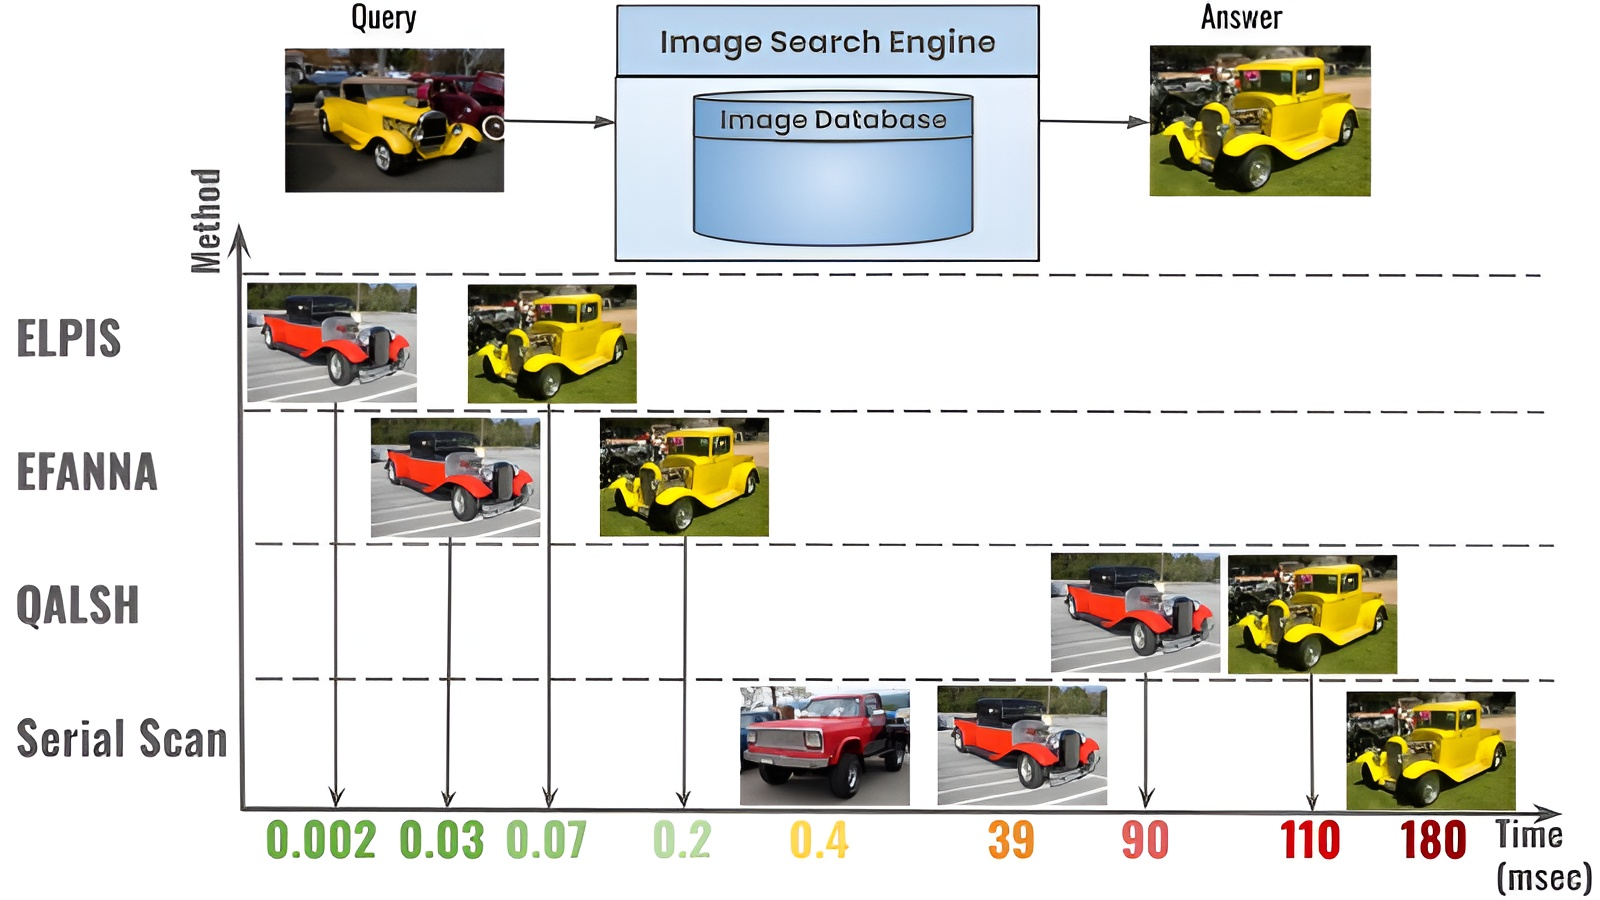
\includegraphics[width=0.8\columnwidth]{../img/intro/ENDTOENDEXAMPLE2.png}
		\caption{
  Image retrieval using different vector search methods.
  }        
		\label{fig:use_case}
 \end{figure}


Figure~\ref{fig:use_case} illustrates vector search in an image retrieval use case. We produce embeddings for ImageNet~\cite{imagenet} using a ResNet50 model~\cite{resnet}. 
We report the time at which a best-so-far (bsf) answer is found (i.e., the image in the database most similar to the query) by vector search techniques from different families: ELPIS~\cite{elpis} and EFANNA~\cite{efanna} for ng-approximate search, QALSH~\cite{qalsh} for $\delta$-$\epsilon$-approximate search, and a serial scan for exact search. 
Each row shows the bsf answer returned by each method (y-axis) at a given timestamp (x-axis). We observe that the graph-based approach  ELPIS returns the same answer as the serial scan and hash-based approach QALSH over three orders of magnitude faster, which explains the popularity of graph-based vector search in many real applications; We also point that not all graph-based methods have the same performance, e.g. ELPIS is 3x faster than EFANNA, 


\section{Main Contributions}
\label{sec:contributions}
Our main contributions are as follows:

\textbf{1. ELPIS: A Scalable Graph-based In-memory Vector Search }  
This thesis introduces \textit{ELPIS}, a novel framework for in-memory \textit{ng}-approximate high-dimensional vector search that combines the strengths of tree-based and graph-based indexing structures. By leveraging the hierarchical organization of trees and summarization of EAPCA-Tree for scalability and the efficiency of graph-based methods for query latency, ELPIS addresses the shortcomings of both approaches. It significantly reduces query latency while maintaining competitive accuracy, even in large-scale datasets comprising billions of high-dimensional vectors. The approach enables ELPIS to scale efficiently with increasing data sizes, making it suitable for modern data-driven applications that require both high speed and accuracy. In extensive evaluations, ELPIS consistently outperforms existing state-of-the-art methods, particularly in latency-sensitive environments.

\textbf{2. Comprehensive Survey and Taxonomy of Graph-Based Search Methods} 
A major contribution of this work is a detailed survey of graph-based similarity search techniques. This survey offers a systematic evaluation of current methods and proposes a new taxonomy that categorizes these approaches into five key paradigms. The taxonomy provides an organized framework for understanding the variety of graph-based methods, clarifying their respective strengths and limitations. This contribution offers researchers and practitioners valuable insights into selecting the most appropriate method for specific applications, while also identifying areas for future exploration. This survey serves as a foundational reference for the community, highlighting challenges in scaling and optimizing graph-based similarity search for increasingly large and complex datasets.

\textbf{3. Throughput Optimization via EAPCA-Based Merging}  
This thesis introduces a novel EAPCA-based merging technique that effectively addresses the throughput limitations of ELPIS. By utilizing Extended Adaptive Piecewise Constant Approximation (EAPCA) lower-bounding distances, the merging process intelligently combines smaller, latency-optimized graphs into larger, throughput-optimized structures. This selective merging approach significantly reduces redundant distance computations during query processing, allowing for more efficient traversal of the vector space. As a result, ELPIS is capable to efficiently balance between latency- and throughput-optimized performance, providing a robust solution for large-scale vector search tasks without the need to build separate indexes optimized for each scenario.

\textbf{3. OIGAS: Optimized Incremental Insertion-based Graph for Efficient Vector Search}  
Expanding upon the findings from the survey, this thesis proposes a novel graph-based search algorithm designed to improve both indexing scalability and query efficiency. The new approach optimizes graph indexing by reducing the required computation to incrementally construct the graph index structures, as well as proposing a combined strategies for pruning edges within the graph based on node in-degree, allowing it to handle large datasets more efficiently than existing techniques. This advancement provides a significant improvement over traditional methods, particularly in scenarios that require a fast indexing of the large collection of data with minimum loss in answer quality during search.


The contributions of this thesis have led to the following publications:

1. Ilias Azizi, Karima Echihabi, Themis Palpanas. Elpis: Graph-Based Similarity Search for Scalable Data Science. Proceedings of the VLDB Endowment 16.6 (2023): 1548-1559.~\cite{elpis}

2. Ilias Azizi, Vector Search on Billion-Scale Data Collections. In VLDB PhD Workshop, 2024.~\cite{iazizi2024}

3. Ilias Azizi, Karima Echihabi, Themis Palpanas. Graph-Based Vector Search:
An Experimental Evaluation of the State-of-the-Art. Proceedings of the ACM on Management of Data (2025).~\cite{gass}

The following contributions are part of ongoing research and are in preparation for future publication:

4. Ilias Azizi, Karima Echihabi, Themis Palpanas. ELPIS+: Optimized Throughput Vector Search over Billion-scale Data Collections. 

5. Ilias Azizi, Karima Echihabi, Themis Palpanas. OIGAS: Optimized Incremental Insertion based Graph for Efficient Vector Search. 

\section{Outline}
The rest of the thesis is organized in 7 chapters. Chapters 2 and 3 lay the foundational background on high-dimensional similarity search, surveys the different families of methods (i.e., tree-based, hash-based, and graph-based), and discusses their strengths and limitations. Chapter 4 introduces a comprehensive taxonomy and analysis of graph-based similarity search methods, evaluating them based on their construction techniques, edge selection strategies, search mechanisms, and scalability. Chapter 5 presents the ELPIS Framework, a hybrid method that integrates tree-based and graph-based structures to optimize both latency and throughput in vector search tasks. Chapter 6 focuses on ELPIS Merging, a novel technique that enhances throughput through an EAPCA-based graph merging approach, providing efficient scalability for billion-scale datasets. Chapter 7 introduces OIGAS, an innovative graph-based method designed for incremental insertion and query performance optimization in dynamic datasets. Each of these chapters includes detailed performance evaluations and comparisons with state-of-the-art methods, supported by experimental results and plots. Finally, Chapter 8 concludes the thesis by summarizing the main contributions and outlining future research directions.
